\documentclass[12pt]{article}

\usepackage{times}
\usepackage{url}
\usepackage{graphicx}
\usepackage{amsmath}
\usepackage{tikz}
\usepackage{float}
\usetikzlibrary{positioning}

\usepackage{color}

\setlength{\textwidth}{6.5in}
\setlength{\textheight}{8.9in}
\setlength{\oddsidemargin}{0.0in}
\setlength{\topmargin}{0.05in}
\setlength{\headheight}{-0.05in}
\setlength{\headsep}{0.0in}

\newcommand{\argmin}{\mathop{\mathrm{argmin}}\limits}
\newcommand{\argmax}{\mathop{\mathrm{argmax}}\limits}

\begin{document}

\begin{center}
{\bf CS 6300} \hfill {\large\bf HW5: Policy Iteration and TD Learning} \hfill {\bf Due February 28, 2017}
\end{center}

\noindent
Please use the \LaTeX\ template to produce your writeups. See the
Homework Assignments page on the class website for details.  Hand in
at: \url{https://webhandin.eng.utah.edu/index.php}.

\section{Policy Iteration (30pts)}

The card game of high-low is played with an infinite deck whose only
cards are 2, 3, and 4 in equal proportion.  You start with one of the
cards showing, and say either {\it high} or {\it low}.  Then a new
card is flipped, and you compare the value of the new card to that of
the old card.

\begin{itemize}

\item If you are right, you get the value of the new card.

\item If the new card has the same value, you don't get any points.

\item If you are wrong, the game is done.

\end{itemize}

\noindent
If you are not done, the new card then becomes the reference card for
drawing the next new card.  You accumulate points as above until you
are wrong and the game ends.

\begin{enumerate}

\item Formulate high-low as an MDP, by listing the states, actions,
  transition rewards, and transition probabilities.  

\begin{center}
\begin{tabular}{cc}
\begin{tabular}{|l|l|l|l|} \hline
$s$ & $a$ & $s'$ & $T(s,a,s')$ \\ \hline
$2$ & $high$ & $win$ & $2/3$ \\ \hline
$2$ & $high$ & $equal$ & $1/3$ \\ \hline
$2$ & $low$  & $lose$ & $2/3$ \\ \hline
$2$ & $low$  & $equal$ & $1/3$ \\ \hline
$3$ & $high$ & $win$   & $1/3$ \\ \hline
$3$ & $high$ & $equal$   & $1/3$ \\ \hline
$3$ & $high$ & $lose$ & $1/3$ \\ \hline
$3$ & $low$ & $win$   & $1/3$ \\ \hline
$3$ & $low$ & $equal$   & $1/3$ \\ \hline
$3$ & $low$ & $lose$ & $1/3$ \\ \hline
$4$ & $high$ & $lose$ & $2/3$ \\ \hline
$4$ & $high$ & $equal$ & $1/3$ \\ \hline
$4$ & $low$  & $win$ & $2/3$ \\ \hline
$4$ & $low$  & $equal$ & $1/3$ \\ \hline
\end{tabular} &
\begin{tabular}{|l|l|}\hline
$s'$       & $R(s')$ \\ \hline
$win$ & $\{2, 3, 4\}$ \\  \hline
$equal$  &  $0$ \\ \hline
$lose$ & $\text{terminate}$  \\ \hline
\end{tabular} \\
Transition Model & Rewards
\end{tabular}
\end{center}

\item You will be doing one iteration of policy iteration.  Assume the
  initial policy $\pi_0(s) = high$.

  \begin{enumerate}

 \item Perform policy evaluation to solve for the utility values
  $V^{\pi_0}(s)$ for the appropriate states $s$.  Please solve these
  equations analytically.

  \[
    V^{\pi_{0}}(s) = \sum_{s^{\prime}}T(s, \pi_{0}, s^{\prime})\left[ R(s, \pi_{0}(s), s^{\prime}) + \gamma V^{\pi_{0}}(s^{\prime}) \right]
  \]

We can also calculate the expected value of drawing a new card by taking the average of the values since they're all equally likely. We assume $\gamma = 1$

\begin{align*}
  V_{k+1}^{\pi_{0}}(2) &= \frac{1}{3}\left(0 + V_{k}^{\pi_{0}}(2)\right) + \frac{1}{3}\left(3 + V_{k}^{\pi_{0}}(3)\right) + \frac{1}{3}\left(4 + V_{k}^{\pi_{0}}(4)\right)\\
\intertext{But we don't know the values for $V_{k}^{\pi_{0}}(3)$ or $V_{k}^{\pi_{0}}(4)$, so we can solve those first and then plug them back into the above equation. We get}
V_{k}^{\pi_{0}}(3) &= \frac{1}{3}(\text{terminate}) + \frac{1}{3}\left(0 + V_{k}^{\pi_{0}}(3)\right) + \frac{1}{3}\left(4 + V_{k}^{\pi_{0}}(4)\right)\\
V_{k}^{\pi_{0}}(4) &= \frac{2}{3}(\text{terminate}) + \frac{1}{3}\left(0 + V_{k}^{\pi_{0}}(4)\right)\\
\intertext{Where we can ignore the termination states as we want to {\em maximize} our output. We can solve for $V_{k}^{\pi_{0}}(4)$ and then $V_{k}^{\pi_{0}}(3)$ to give}
V_{k}^{\pi_{0}}(4) &= 0\\
V_{k}^{\pi_{0}}(3) &= \frac{1}{3}\left( 0 + V_{k}^{\pi_{0}}(3)\right) + \frac{1}{3}\left( 4 + V_{k}^{\pi_{0}}(4)\right)\\
                &= \frac{1}{3}V_{k}^{\pi_{0}}(3) + \frac{4}{3}\\
                &= 2\\
\intertext{Finally, by solving for $V_{k}^{\pi_{0}}(2)$}
V_{k+1}^{\pi_{0}}(2) &= \frac{1}{3}\left( 0 + V_{k}^{\pi_{0}}(2)\right) + \frac{1}{3}\left( 3 + V_{k}^{\pi_{0}}(3)\right) + \frac{1}{3}\left( 4 + V_{k}^{\pi_{0}}(4)\right)\\
                &= \frac{9}{2}
\end{align*}

  \item Perform policy improvement to find the next policy $\pi_1(s)$.

    The equation for calculating the next policy is
    
\begin{align*}
  \pi_{k+1}(s) &= \argmax_{a} \sum_{s^{\prime}} T(s,a,s^{\prime})\left[ R(s,a,s^{\prime}) + \gamma V_{k}^{\pi_{k}}(s^{\prime}) \right]
  \intertext{We can use this to find the next policy update for each state, giving}
  \pi_{1}(2) &= \argmax_{a} \left\{ \begin{array}{c c c c}\frac{1}{3}\left(0 + \frac{9}{2}\right)  & = & 3/2 & (low)\\
      \frac{1}{3}\left(0 + \frac{9}{2}\right) + \frac{1}{3}\left(3 + 2\right) + \frac{1}{3}\left(4 + 0\right)  & = & 27/6 & (high)\end{array}\right.\\
  \pi_{1}(2) &= high\\
  \pi_{1}(3) &= \argmax_{a} \left\{ \begin{array}{c c c c}\frac{1}{3}\left(0 + 2\right) + \frac{1}{3}\left(2 + \frac{9}{2}\right) & = & 17/6 & (low)\\
      \frac{1}{3}\left(0 + 2\right) + \frac{1}{3}\left(4 + 0\right) & = & 2 & (high)\end{array}\right.\\
  \pi_{1}(3) &= low\\
  \pi_{1}(4) &= \argmax_{a} \left\{ \begin{array}{c c c c}\frac{1}{3}\left(2 + \frac{9}{2}\right) + \frac{1}{3}\left(3 + 2\right) + \frac{1}{3}(0 + 0)  & = & 23/6 & (low)\\
      \frac{1}{3}(0 + 0)  & = & 0 & (high)\end{array}\right.\\
  \pi_{1}(4) &= high
\end{align*}

  \end{enumerate}

\end{enumerate}

\clearpage

\section{Life as a Student}

Jennifer is currently finishing up in college and is trying to decide
what she wants to do with the rest of her life.  She sketches her
options as a known MDP:

\begin{center}
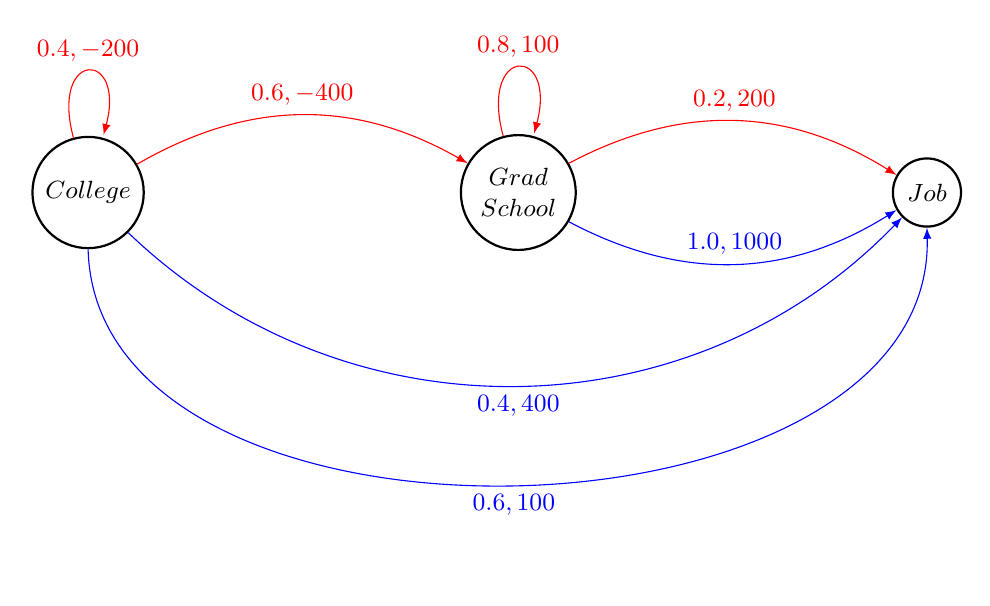
\begin{tikzpicture}[auto,node distance=8mm,>=latex,font=\small]

\tikzstyle{round}=[thick,draw=black,circle]

    \node[round] (C) {$College$};
    \node[round,right=40mm of C, align=center] (G) {$Grad$\\ $School$};
    \node[round,right=40mm of G, align=center] (J) {$Job$};

\path
    (C) edge[loop above, red] node{$0.4,-200$}  (C)
    (C) edge[->, bend left, red] node[above]{$0.6,-400$}  (G)
    (C) edge[->, bend right, blue, out=-45, in=-135] node[below]{$0.4,400$} (J)
    (C) edge[->, bend right, blue, out=-90, in=-90] node[below]{$0.6,100$} (J)
    (G) edge[->, loop above, red] node[above]{$0.8, 100$} (G)
    (G) edge[->, bend left, red] node[above]{$0.2, 200$} (J)
    (G) edge[->, bend right, blue] node[above]{$1.0, 1000$} (J);
\end{tikzpicture}
\end{center}

\vspace{-2.5em}
At each point in her life she can choose to either continue in school
(action {\color{red}{$x$}}) or try to get a job (action {\color{blue}{$y$}}).  Her three states are
{\bf C}ollege, {\bf G}rad School and {\bf J}ob.  {\bf J} is a terminal
state.  Transition probabilities $t$ and immediate rewards $r$ are
shown on the arcs as $t,r$.  The discount $\gamma = 0.5$.

\begin{enumerate}

\item Using value iteration, compute values for each state.  Add or
  remove extra lines for iteration as needed.

\begin{center}
\begin{tabular}{|l|r|r|} \hline
$i$ & $V_i^*(C)$ & $V_i^*(G)$ \\ \hline
$0$ &$0.0$ &$0.0$ \\ 
$1$ & $220.0$ & $1000.0$\\ 
$2$ & $220.0$ & $1000.0$\\ 
\hline
\end{tabular}
\end{center}

The non-linear equation for {\em Value Iteration} is defined as

\[
  V^{*}_{k+1}(s) = \max_{a}\sum_{s^{\prime}}T(s, a, s^{\prime})\left[ R(s, a, s^{\prime}) + \gamma V^{*}_{k}(s^{\prime})\right]
\]

We can calculate the value of $V$ for two iterations of $College$.

\begin{align*}
V_{1}^{*}(C) &= \max_{a}\left\{ \begin{array}{lcr@{}}
                                  0.4(-200 + 0) + 0.6(-400 + 0) & = -320 & ({\color{red}{x}})\\
                                  0.4(400 + 0) + 0.6(100 + 0) & = \phantom{-}220 & ({\color{blue}{y}})\\
                                \end{array}\right.\\
V_{2}^{*}(C) &= \max_{a}\left\{ \begin{array}{lcr@{}}
                                  0.4(-200 + 0.5(220)) + 0.6(-400 + 0.5(220)) & = -210& ({\color{red}{x}})\\
                                  0.4(400 + 0.5(0)) + 0.6(100 + 0.5(0)) & = \phantom{-}220 & ({\color{blue}{y}})\\
                                \end{array}\right.
\end{align*}

\item Suppose Jennifer didn't actually know the values of the MDP.
  Instead, she watched three of her older siblings go through life.
  They exhibited the following trajectories:

\begin{center}
\begin{tabular}{|l|l|l|} \hline
{\bf Sibling 1} & {\bf Sibling 2} & {\bf Sibling 3} \\ \hline
$C, {\color{red}{x}}, -200$ & $C, {\color{red}{x}}, -400$ & $C, {\color{red}{x}}, -400$ \\
$C, {\color{red}{x}}, -200$ & $G, {\color{red}{x}},  \phantom{-}100$ & $G, {\color{red}{x}},  \phantom{-}100$ \\
$C, {\color{blue}{y}}, \phantom{-}400$ & $G, {\color{red}{x}},  \phantom{-}100$ & $G, {\color{red}{x}},  \phantom{-}100$ \\
$J$          & $G, {\color{blue}{y}}, \phantom{-}1000$ & $G, {\color{red}{x}},  \phantom{-}200$ \\
             & $J$          & $J$          \\ \hline
\end{tabular}
\end{center}

  \begin{enumerate}

  \item According to direct estimation, what are the transition
    probabilities $T(C,{\color{red}{x}},C)$, $T(C,{\color{red}{x}},G)$ and $T(C,{\color{blue}{y}},J)$?

    \begin{table}[H]
      \centering
      \begin{tabular}{c c c}
        \hline\hline
        $T(C,{\color{red}{x}},C)$ & $T(C,{\color{red}{x}},G)$ & $T(C,{\color{blue}{y}},J)$\\
        \hline
        $4/9$ & $5/9$ & $1/2$\\
        \hline
       \end{tabular}
      \end{table}

  \item According to direct estimation, what are the rewards
    $R(C,{\color{red}{x}},C)$, $R(C,{\color{red}{x}},G)$ and $R(C,{\color{blue}{y}},J)$?


    \begin{table}[H]
      \centering
      \begin{tabular}{c c c}
        \hline\hline
        $R(C,{\color{red}{x}},C)$ & $R(C,{\color{red}{x}},G)$ & $R(C,{\color{blue}{y}},J)$\\
        \hline
        $-300$ & $120$ & $400$\\
        \hline
       \end{tabular}
      \end{table}


  \item Use TD Learning instead to find estimates of the value
    function $V^{\pi}(s)$, assuming $\alpha=0.5$.

    The equation for Temporal Difference Learning is

    \begin{align*}
      V^{\pi}(s) &\leftarrow (1 - \alpha)V^{\pi}(s) + \alpha\left[R(s,\pi,s^{\prime}) + \gamma V^{\pi}(s^{\prime}) - V^{\pi}(s)\right]
    \end{align*}

  \end{enumerate}

\end{enumerate}

\end{document}
